\newpage		
	\section*{Лист 2}
		\subsection*{2.1}
		Заметим, что $f(x,y) = Ax^2 + Bxy + Cy^2$, а $g(f)$ геодезическая с основаниями в корнях $Ax^2 + Bx + C$, то есть геодезическая однозначно задана 2 точками.\\
		Тогда докажем, что $f \to g(f)$ -- сюръекция.\\
		Заметим, что $f$ не может соответствовать более чем одной геодезической, так как это значило бы, что через данные 2 точки можно провести более одной геодезической, что не так.\\
		Заметим также что каждой геодезической соответствует хотя бы одна функция $f$, так как если геодезическая вертикальная с основанием в точке $\alpha$, то она ей соответствует функция $x^2 + 2\alpha x + \alpha^2$, если же это обычная геодезическая с основаниями $x_1, x_2$, то ей соответствует функция $x^2 - (x_1 + x_2)x + x_1x_2$.\\
		так мы доказали что это сюръекция\\
		\\
		Теперь докажем что $g(f) = g(\tilde{f}) \Leftrightarrow \tilde{f} = \lambda f,\ \lambda \in \mathbb{R}$.\\
		Заметим что если $g(f) = g(\tilde{f})$, то геодезические, а следовательно и их основания, совпали, откуда следует что корни $f$ и $\tilde{f}$ совпадают. то есть $f = (x - x_1)(x - x_2)$ и $\tilde{f} = f_1(x)(x - x_1)(x - x_2)$, осталось заметить, что $\deg(\tilde{f}) = 2$, откуда следует что $f_1(x) = \lambda,\ \lambda \in \mathbb{R}$.\\
		А из $\tilde{f} = \lambda f$ очевидно следует равенство $g(f) = g(\tilde{f})$, так как при домножении на $\lambda \in \mathbb{R}$ корни уравнения не меняются.
		
		\subsection*{2.2}
		\begin{figure}[h]
			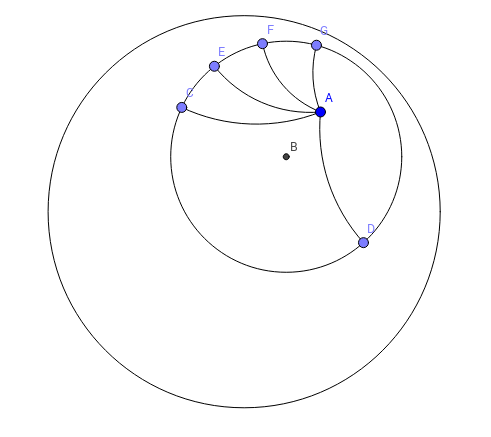
\includegraphics[width=0.5\linewidth]{pic8}
		\end{figure}
		\noindent
		Пусть $g_1(f)$ -- операция приводящая $f(p,q)$ к $f(\tilde{f},0)$, то есть сопоставляющая $f(p,q)$ функцию, с корнями совпадающими с основаниями геодезической, также можно заметить что эта функция -- инъекция. 
		Тогда
		\begin{gather*}
			f = f(p,q) = Ap^2 + Bpq + Cq^2\\
			g_1(f) = g_1(f(p,q)) = f(\tilde{p}, 0) = A\tilde{p}^2 + B\tilde{p} + C\\
			A\tilde{p}_1^2 + B\tilde{p}_1 + C = A\tilde{p}_2^2 + B\tilde{p}_2 + C = 0\\
			A \in \text{GL}(2,\mathbb{R})\\
			A = 
			\begin{pmatrix}
				a_1 & a_2\\
				a_3 & a_4
			\end{pmatrix}\\
		\end{gather*}
		Откуда
		\begin{gather*}
			A^{-1} = 
			\frac{1}{a_1a_4 - a_2a_3}
			\begin{pmatrix}
				a_4 & -a_2\\
				-a_3 & a_1
			\end{pmatrix}\\
			f \circ A^{-1} (p,q) = f\Bigg((p,q) \cdot 
			\begin{pmatrix}
				a_4 & -a_2\\
				-a_3 & a_1
			\end{pmatrix}\Bigg)
			=
			f(pa_4-qa_2, qa_1 - pa_3)\\
		\end{gather*}
		Мы выкинули дробь $\frac{1}{a_1a_4 - a_2a_3}$ так как она не влияет на корни, а следовательно и на геодезическую.\\
		Теперь рассмотрим
		\begin{gather*}
			f(pa_4-qa_2, qa_1 - pa_3) = 0\\
			g_1(f(pa_4-qa_2, qa_1 - pa_3)) = f(p'a_4-a_2, a_1 - p'a_3)\\
			A(p'a_4 - a_2)^2 + B(p'a_4 - a_2)(a_1 - p'a_3) + C(a_1 - p'a_3)^2 = 0\\
			A\Bigg(\frac{p'a_4 - a_2}{a_1 - p'a_3}\Bigg)^2 + B\frac{p'a_4 - a_2}{a_1 - p'a_3} + C = 0\\
			\frac{p'a_4 - a_2}{a_1 - p'a_3} = \frac{-B \pm \sqrt{B^2 - 4AC}}{2A}\\
			(p'a_4 - a_2) = (a_1 - p'a_3) \cdot \frac{-B \pm \sqrt{B^2 - 4AC}}{2A}\\
			(p'a_4 - a_2) = (a_1 - p'a_3) \cdot \tilde{p}_{1,2}\\
			p'a_4 - a_2 = a_1\tilde{p}_{1,2} - p'a_3\tilde{p}_{1,2}\\
			p'a_4 +	p'a_3\tilde{p}_{1,2} = a_1\tilde{p}_{1,2} + a_2\\
			p'= \frac{a_1\tilde{p}_{1,2} + a_2}{a_3\tilde{p}_{1,2} + a_4}
		\end{gather*}
		Откуда следует верность коммутативной диаграммы




		\subsection*{2.3}
		Рассмотрим орицикл $q=0$.\\
		Заметим, что если $g(f)$ -- геодезическая, один из концов которой является $\infty$, то для нее выполнено:
		\begin{gather*}
			d(O\Big(\frac{p}{q}\Big), g(f)) = \log\frac{|f(p,q)|}{\sqrt{B^2 - 4AC}}
		\end{gather*}
		А ткаже можно заметить что расстояние между корнями уравнения $Ax^2 + Bx + C = 0$ это
		\begin{gather*}
			\frac{2p^2 \sqrt{B^2 - 4AC}}{|Ap^2|}
		\end{gather*}
		И, соответственно, высота геодезической с основаниями в этих корнях
		\begin{gather*}
			\frac{p^2 \sqrt{B^2 - 4AC}}{|Ap^2|}
		\end{gather*}
		Теперь рассмотрим общий случай и приведем его к случаю $q=0$\\
		\begin{gather*}
			d(O\Big(\frac{p}{q}\Big), g(f)) = \\
			\\
			d(M_{A}O\Big(\frac{p}{q}\Big), M_{A} g(f)) = \\
			\\
			d(O\Big(\frac{\tilde{p}}{0}\Big), g(f \circ A^{-1})\Big) = \\
			\\
			\log \frac{|f \circ A^{-1}\ (\tilde{p}, 0)|}{\sqrt{B^2 - 4 AC} \circ A^{-1}} = \\
			\\
			\log\frac{|f(p,q)|}{\sqrt{B^2 - 4AC}}
		\end{gather*}